\vspace{-15pt}
\begin{figure}[h]
    \centering
    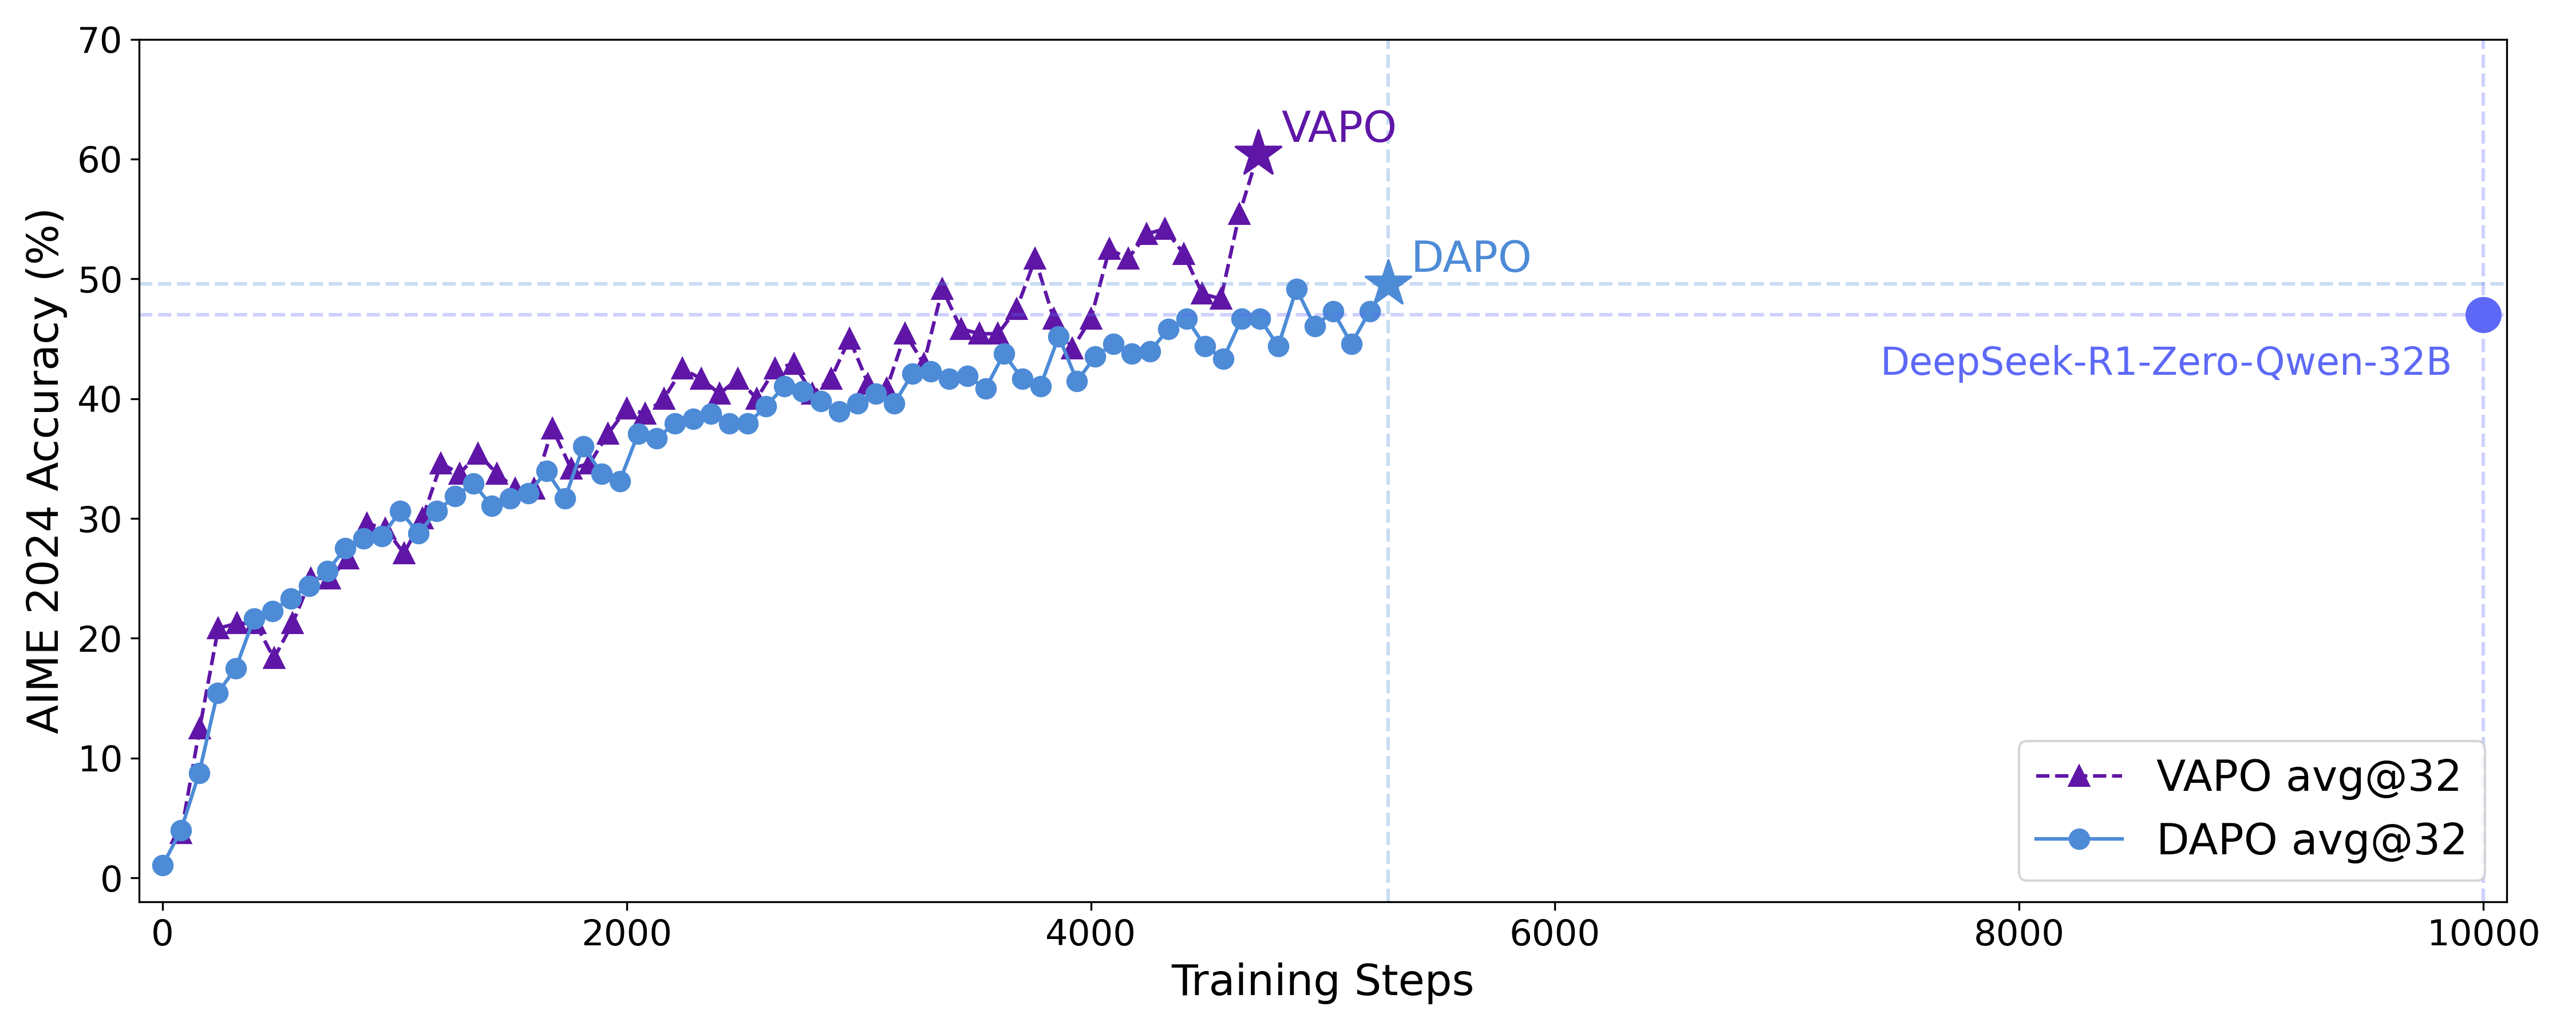
\includegraphics[width=0.85\linewidth]{fig/score.png}
    \caption{AIME 2024 scores of \textbf{VAPO} on the Qwen2.5-32B base model, demonstrates significant superiority over the previous state-of-the-art (SOTA) method DAPO, achieving this with notably fewer training steps. The x-axis denotes the gradient update steps.
    }
    \label{fig:front}
\end{figure}

\section{Introduction}

% Start by inserting a figure: Figure 1 compares VAPO, DAPO, and PPO. 

% To frame the discussion, current approaches primarily rely on algorithms lacking a value model, which often suffer from low efficiency. Highlight the advantages of PPO-based improvements—such as enhanced stability and sample efficiency 

% introducing the key modifications proposed in this work.
%\subsection{Hello World}
Reasoning models~\cite{gemini-thinking,qwq,k1.5} such as OpenAI O1 \citep{o1} and DeepSeek R1 \citep{deepseekai2025deepseekr1incentivizingreasoningcapability} have significantly advanced artificial intelligence by exhibiting remarkable performance in complex tasks such as mathematical reasoning, which demand step-by-step analysis and problem-solving through long chain-of-thought (CoT)~\cite{cot_2022} at test time.
Reinforcement learning (RL) plays a pivotal role in the success of these models~\cite{k1.5,areal,dapo,shao2024deepseekmath,hu2025reinforce++,rloo,ahmadian2024basicsrevisitingreinforcestyle,sutton1998rl}. It gradually enhances the model's performance by continuously exploring reasoning paths toward correct answers on verifiable problems, achieving unprecedented reasoning capabilities.


In the Large Language Models (LLM)~\cite{gpt3,gpt4,dsv3,grok,team2023gemini,claude35sonnet,chowdhery2023palm} RL training, value-model-free methods like GRPO~\cite{shao2024deepseekmath} and DAPO~\cite{dapo} have demonstrated remarkable effectiveness. These approaches eliminate the computational overhead of learning a value model, instead computing advantage solely based on the final reward of the entire trajectory. The trajectory-level advantage is then directly assigned as the token-level advantage for each position in the sequence. When training a reliable value model is particularly challenging, value-model-free methods deliver an accurate and stable baseline for advantage calculation by averaging the rewards across multiple trajectories within a group. This group-based reward aggregation mitigates the need for explicit value estimation, which often suffers from instability in complex tasks. Consequently, value-model-free methods have gained significant traction in addressing difficult problems such as long-CoT reasoning, with substantial research efforts focused on optimizing their frameworks.

Despite the notable success achieved by the value-model-free methods, we argue that value-model-based approaches possess a higher performance ceiling if the challenges in training value models can be addressed. First, value models enable more precise credit assignment by accurately tracing the impact of each action on subsequent returns, facilitating finer-grained optimization~\cite{ppo}. This is particularly critical for complex reasoning tasks, where subtle errors in individual steps often lead to catastrophic failures, and it remains challenging for model optimizing under value-model-free frameworks~\cite{vc-ppo}. Secondly, in contrast to the advantage estimates derived from Monte Carlo methods in value-model-free approaches, value models can provide lower-variance value estimates for each token, thereby enhancing training stability. Furthermore, a well-trained value model exhibits inherent generalization capabilities, enabling more efficient utilization of samples encountered during online exploration. This significantly elevates the optimization ceiling of reinforcement learning algorithms. Consequently, despite the formidable challenges in training value models for complex problems, the potential benefits of overcoming these difficulties are substantial.

However, training a perfect value model in Long COT tasks presents significant challenges.
First, learning a low-bias value model is non-trivial given the long trajectory and the instability of learning value in a bootstrapped way. Second, handling both short and long responses simultaneously is also challenging, as they might exhibit very distinct preferences towards the bias-variance trade-off during optimization. Last but not least, the sparsity of the reward signal from verifiers is further exacerbated by the long CoT pattern, which intrinsically requires better mechanisms to balance exploration and exploitation. To address the aforementioned challenges and fully unleash the potential of value-model-based methods in reasoning tasks, we present \textbf{V}alue \textbf{A}ugmented proximal \textbf{P}olicy \textbf{O}ptimization (\textbf{VAPO}), a value-model-based RL training framework. VAPO draws inspiration from prior research works such as VC-PPO~\cite{vc-ppo} and DAPO~\cite{dapo}, and further extends their concepts.

We summarize our key contributions as follows:
\begin{enumerate}
\item We introduce VAPO, the first value-model-based RL training framework to outperform value-model-free methods on long COT tasks significantly. VAPO not only demonstrates remarkable superiority in terms of performance but also showcases enhanced training efficiency, streamlining the learning process and underscoring its potential as a new benchmark in the field.
\item We propose Length-adaptive GAE, which adaptively adjusts the $\lambda$ parameter in GAE computation based on response lengths. By doing so, it effectively caters to the distinct bias-variance trade-off requirements associated with responses of highly variable lengths. As a result, it optimizes the accuracy and stability of the advantage estimation process, particularly in scenarios where the length of the data sequences varies widely.
\item We systematically integrate techniques from prior work, such as Clip-Higher and Token-level Loss from DAPO \citep{dapo}, Value-Pretraining and Decoupled-GAE from VC-PPO \citep{vc-ppo}, self-imitation learning from SIL \citep{SIL}, and Group-Sampling from GRPO \citep{shao2024deepseekmath}. Additionally, we further validate their necessity through ablation studies.
\iffalse
    \item In the context of CoT reasoning, value model bias hinders the effective training of value-model-based models. To address this, we propose a \textbf{Length-Adaptive GAE} method and adopt the decoupling Generalized Advantage Estimation (GAE) and value warm-up from VC-PPO~\cite{vc-ppo} to facilitate stable value learning. Experimental results validate our hypothesis, showing that without these techniques, the model fails to achieve satisfactory performance. 
    \item  Long-time training negatively impacts the model's exploration ability. To counter this, we follow DAPO~\cite{dapo} using the CLIP, encouraging more extensive exploration in later stages of training. Experimental results also show that this adjustment leads to significant performance improvements.
\fi
\end{enumerate}
 \textbf{VAPO} is an effective reinforcement learning system that brings together these improvements. These enhancements work together smoothly, leading to a combined result that’s better than the sum of the individual parts. 
 We conduct experiments using the Qwen2.5-32B pre-trained model, ensuring no SFT data is introduced in any of the experiments, to maintain comparability with related works (DAPO and DeepSeek-R1-Zero-Qwen-32B).
 The performance of \textbf{VAPO} improves from vanilla PPO a score of 5 to 60, surpassing the previous SOTA value-model-free methods DAPO~\cite{dapo} by 10 points. More importantly, \textbf{VAPO} is highly stable — we don't observe any crashes during training, and the results across multiple runs are consistently similar.


\iffalse
In this paper, we present \textbf{V}alue \textbf{A}ugmented proximal \textbf{P}olicy \textbf{O}ptimization (\textbf{VAPO}), a value-model-based RL training framework. \textbf{VAPO} addresses the challenges of value model training in long-CoT tasks while maximizing the benefits that value models offer to RL algorithms. 
The main differences between reasoning models and traditional RLHF methods lie in two key aspects: (a) The introduction of long CoT significantly increases the sequence length, often tens of times longer than that of traditional models. (b) Since the reward are given by a verifier instead of a model, reward hacking is not a concern, allowing for much longer training, typically tens of times more steps compared to conventional approaches.
The long sequences introduce bias into the reward model, particularly due to reward discounting. A more effective reward learning approach is thus needed.
And  the longer training  leads to a collapse in exploration during later stages, necessitating enhanced exploration mechanisms.
To address this issue, we draw inspiration from prior work~\cite{vc-ppo,dapo} and propose our system approach as follows.
\fi
%We aim to explore the limits of VAPO and also conduct a systematic study of a few methods proposed in prior work.
%Concurrently, VAPO integrates established strategies from prior literature to enhance the efficiency of exploration and exploitation during RL training. 
%The specific improvement strategies are as follows:
% During the RL training phase, GRPO is widely employed and achieves favorable results in balancing model training effectiveness and training resource consumption. However, due to the absence of a value model, GRPO is unable to perform fine-grained token-level policy optimization. This limitation not only restricts the model's exploration capabilities but also reduces its training efficiency. To address this, DAPO introduces a higher clip strategy and dynamic sampling to mitigate issues of insufficient exploration and low training efficiency. Nevertheless, these approaches cannot fundamentally resolve the core problems inherent in GRPO. In contrast, a more promising alternative is to adopt PPO, as exemplified in OpenAI's o series models. However, applying the PPO algorithm to long COT generation scenarios is non-trivial, primarily facing two key challenges: 1) How to efficiently train a value model to enable accurate predictions on long text sequences; 2) How to balance exploration and exploitation to improve optimization efficiency, which is particularly crucial in scenarios with high resource consumption for long COT models.

% In this paper, we propose Value Augmented proximal Policy Optimization (VAPO), a novel RL framework designed to address the aforementioned challenges of PPO in long CoT tasks. VAPO enhances the standard PPO framework through seven key technical innovations:  

%\begin{enumerate}
%\item \textbf{Value Model Pretraining}, a dedicated pretraining stage for the value model to rectify estimation biases inherent in value initialization.  
%\item \textbf{Decoupled Generalized Advantage Estimation (Decoupled-GAE)}, which reduces advantage estimation variance while maintaining unbiased optimization objectives for the value model.  
%\item \textbf{Adaptive GAE}, which dynamically adjusts the $\lambda$ parameter in GAE based on sequence length during policy optimization, mitigating reward signal decay in long sequences.  
%\item \textbf{Clip-Higher Strategy}, which expands the policy optimization scope to include more tokens with lower sampling probability to enhance model exploration.  
%\item \textbf{Token-Level Policy Gradient Loss}, which ensures balanced gradient contributions from each token in long sequences, strengthening the suppression of erroneous reasoning patterns.  
%\item \textbf{Positive Example LM Loss}, which improves the exploitation efficiency of high-quality responses.
%\item \textbf{Rebalance Generation Budget}, which reduces the number of prompts per generation run while increasing the number of responses generated per prompt. Additionally, incorporating more detailed contrastive signals enhances the granularity of comparisons.
%\end{enumerate} 


%Through the aforementioned enhancements, VAPO dramatically enhances training stability, evidenced by the steady evolution of generated sequence lengths and consistent improvement in test set metrics throughout the training process. Furthermore, VAPO demonstrated significantly superior training efficiency compared to DAPO. Under the same learning rate, VAPO achieved superior performance using only 70\% of the training steps required by DAPO. On the AIME24, VAPO achieves 53.3, significantly outperforming DAPO (46.7\footnote{DAPO \cite{dapo} achieved 50.0 on a new training set, while we conduct comparisons on the old training set}) and the original PPO baseline (???). And our ablation studies demonstrate that all of the six techniques contribute to the improvement of model performance.